\chapter{Bistable Helical Origami Gripper for Sensor Placement on Branches}
\label{ch:origami_gripper}

\author{Christian Geckeler*}
\author{Stefano Mintchev}

\begin{affiliations}
Christian Geckeler and Prof. Dr. Stefano Mintchev\\
Swiss Federal Institute of Technology Zürich\\
Universitätstrasse 2\\
8092 Zürich\\
Switzerland\\
Email Address: christian.geckeler@usys.ethz.ch\\~\\ % cgeckeler@ethz.ch

Swiss Federal Institute for Forest, Snow and Landscape Research WSL\\
Zürcherstrasse 111\\
8903 Birmensdorf\\
Switzerland\\~\\

\end{affiliations}


\begin{abstract} % exactly 199
Understanding forest functioning is limited by the scalability of monitoring solutions and difficulty of access. Manual sensor placement can reach most locations but lacks scalability. Micro aerial vehicles (MAVs) allow for scalable sensor delivery, but current solutions are limited to attaching sensors to the trunk or large branches with spines or adhesives. The thinner branches of the outer canopy remain inaccessible, despite being of particular interest due to the important physiological processes occurring in the foliage. In this work, a MAV-deployable bistable helically coiling origami gripper is developed. The unfurled state allows for transport with a MAV, and when pushed against a branch triggers the second helically coiled state, which permits secure attachment to branches. Origami manufacturing keeps the weight of the gripper below 5g, despite holding up to 280g, and gripping diameters from 8mm to 38mm inclined up to 30\degree. The holding force, activation force, and resistance to tilt and rotation offsets are experimentally characterized. The deployment and retrieval of the gripper and sensor are demonstrated outside, where sensor data is collected from previously inaccessible branches in the outer canopy. Enabling robust sensor attachment in the outer canopy marks a step towards scalable environmental monitoring of forest ecosystems.

 
\end{abstract}


\section{Introduction}

Lack of high spatial and temporal resolution data hampers understanding and restoration of natural ecosystems. This is a long-standing challenge in forest canopies. Despite being a biodiversity hotspot \cite{Nakamura2017}, \cite{Ozanne2003d} and providing crucial ecosystem services (e.g. carbon sequestration \cite{Harris2012}, \cite{Didham2004}, nutrient cycling \cite{CE2002}, and climate regulation \cite{Ellison2012}), the access and study of canopies is often unsafe and expensive, requiring experienced climbers or the use of forklifts and cranes \cite{Parker1992}. For example, forest canopies create a buffering effect on the local humidity, temperature, and light conditions beneath them: the microclimate \cite{Nakamura2017}. Microclimates are particularly important within the context of understanding, measuring, and mitigating climate change \cite{Frenne2021}, \cite{Zellweger2020}, \cite{VonArx2012}. However, many open research questions remain \cite{Jucker2020},\cite{Bachofen2020}, \cite{Law2020}, and finding the answers would require a dense network of sensors to record high resolution climate data.
\begin{figure} [htbp]
    \centering
    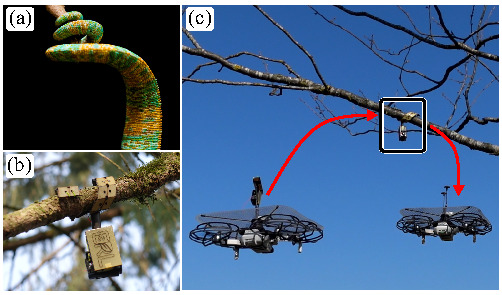
\includegraphics{figs/fig_1_all-in-one/Figure_1.pdf}
    \caption{Natural and artificial helical grippers. (a) Example of helical coiling in nature (Image by Ante Hamersmit on Unsplash). (b) The proposed origami helical gripper coiled around a branch with a sensor box attached to it. (c) Composition of the gripper and sensor delivery with a MAV.}
    \label{fig:bio-inspiration}
\end{figure}

Placing many sensors in such unsafe and difficult to access environments is a relevant application for Micro Aerial Vehicles (MAVs). MAVs are gradually demonstrating flight in forests \cite{Mulgaonkar2018b}, \cite{Tan2017}, \cite{Zheng2020}, and the ability to deliver sensors on surfaces for non-destructive testing of infrastructures \cite{Gonzalez-deSantos2019}, \cite{Ikeda2017}, \cite{Bodie2019}. In the latter application, aerial robots transport contact sensors that are pressed and dragged across the surfaces of infrastructures, but not attached to them. Exceptions are \cite{Jarvis2018}, where a sensor with a magnetic latch is attached to a steel pipe, and \cite{McArthur2018b}, where double-sided adhesives are used to attach sensors on vertical surfaces. The few examples of sensor delivery in canopies include firing sensor darts from aerial robots \cite{Farinha2020}, and placing adhesive sensors with an aerial manipulator \cite{Hamaza2019}. Whereas the aforementioned approaches were successfully demonstrated on tree trunks or large branches, their use is not directly transferable to thin and flexible branches. Thin branches, which are also susceptible to swaying in the wind, are difficult to target with darts; their flexibility also makes it difficult to use adhesives or spines that need to be pressed onto or into the wood \cite{Farinha2020}. This is a significant limitation because the outer and most flexible branches are the site of important photosynthetic activity, gas exchange, and water transpiration, and therefore a core target for environmental sensors.

Currently, reliable canopy access is limited to human climbers manually attaching sensors \cite{Anderson2020a}, \cite{Didham2014}, \cite{Cannon2021}, such as by physically tying them to branches with ropes or zip ties. This type of dexterous manipulation for robots is very complicated, particularly when attempted with a aerial robot. In nature, coiling is a simple but effective method of grasping based on elongated prehensile appendages (see \textbf{Figure \ref{fig:bio-inspiration}a}), e.g. giraffe tongues, monkey, lizard, and seahorse tails, cephalopod tentacles, elephant trunks, and tendrils in plants. Inspired by these versatile appendages, researchers have developed helical grippers exploiting different manufacturing and actuation technologies, including pneumatic \mbox{\cite{Kumar2018}}, \mbox{\cite{Hu2020}}, \mbox{\cite{Pal2020ElasticMachines}}, hydraulic \mbox{\cite{Galloway2016}}, \mbox{\cite{Hoang2020a}}, cable-actuated \mbox{\cite{Mazzolai2019}}, magnetic \mbox{\cite{Wu2021StretchableTwisting}}, electric \mbox{\cite{Meder2022AArrangement}}, \mbox{\cite{Shao2018BioinspiredActuators}} or thermal-actuated systems \mbox{\cite{Wang2018}}. For a detailed treatment of soft grippers, the reader is referred to \mbox{\cite{Shintake2018SoftGrippers}} and \mbox{\cite{Chi2022}}. Most of these grippers use actuators to grasp multiple times, but this additional complexity and weight is not necessary for a gripper that needs to be activated only a single time to attach to a branch. Therefore, a passively-actuated bistable mechanism is developed, which dispenses with bulky actuators and fits the task while offering a lighter design. Compared to claws or multi-fingered manipulators, helical grippers are better suited for applications that require high conformability or high-load sustainability \cite{Hoang2020a}. The helical grasp with elongated appendages is particularly effective for gripping slender, rounded objects of different sizes and orientations, thereby making this solution well suited for gripping branches. Additionally, the high-load sustainability is conducive to lightweight grippers that can be transportable by small aerial robots suited to fly in dense vegetation.

Aerial deployment, particularly with MAVs, place limitations on the size and weight of deployable structures. Origami provides a method of producing lightweight 3D structures from folding 2D planar sheets. Using a composite of stiff and flexible materials enables the creation of rigid substructures with flexible joints, allowing for dynamic structures such as snapping rings \cite{Wu2021}, wings \cite{Baek2020}, rotating propeller guards \cite{Sareh2018}, morphing wheels \cite{Lee2021}, haptic interfaces \cite{Mintchev2019}, and grippers \cite{Li2019d}, \cite{Mintchev2018}, \cite{Faber2018a}, \cite{Firouzeh2017a}, \cite{Boyvat2017}, \cite{Kim2018c}. Therefore, origami presents a scalable and lightweight manufacturing method for aerially deployable structures.

Here, a novel bistable helical origami gripper is presented (Figure \ref{fig:bio-inspiration}b), capable of being deployed with an  aerial robot to attach a sensor payload to branches (Figure \ref{fig:bio-inspiration}c). The bistability of the gripper allows it to be transported in an unfurled state and then snap to coil around a branch when pressed against it.

There are three main contributions of this work to the fields of gripper design and sensor placement. First, we present a novel bistable helically coiling origami gripper capable of attaching to cylindrical objects between the diameters of 8 mm to 38 mm. Through origami manufacturing and passive bistable actuation, mechanical and actuation complexity can be avoided. The result is a 5-gram MAV transportable helical structure that allows secure gripping of branches with diameters up to 38 mm inclined up to \mbox{30\degree}, sustaining up to 2.8 N, which is more then 50 times its own weight. Second, the gripper is geometrically and experimentally characterized. The effect of the adjustable gripper parameters; length, width, segment angle, and number of segments, on the gripper attributes; minimum and maximum graspable diameters, coiled length, and gap between coils, are analyzed geometrically. This allows the gripper to be tuned according to user specifications, for example, changing the gripper dimensions to grasp a certain diameter. Experiments demonstrate the maximum holding force, the activation force, and the robustness of the gripper to tilt and rotation offsets during activation. Third, we demonstrate the utility of the bistable helical origami gripper by deploying and collecting sensors with a MAV from the previously inaccessible thin branches of the outer canopy in several outdoor demonstrations. To re-collect the sensor a sensor box is developed which releases tension in the elastic of the gripper and allows it to be collected with a MAV when this is magnetically attached to it. While previous approaches were able to attach sensors to tree trunks and thick branches, to the best of the authors' knowledge this work is the first solution to attach sensors the thinner branches of the outer canopy, which are of particular interest to study tree physiology.


\section{Results}

\begin{figure} [htbp]
    \centering
    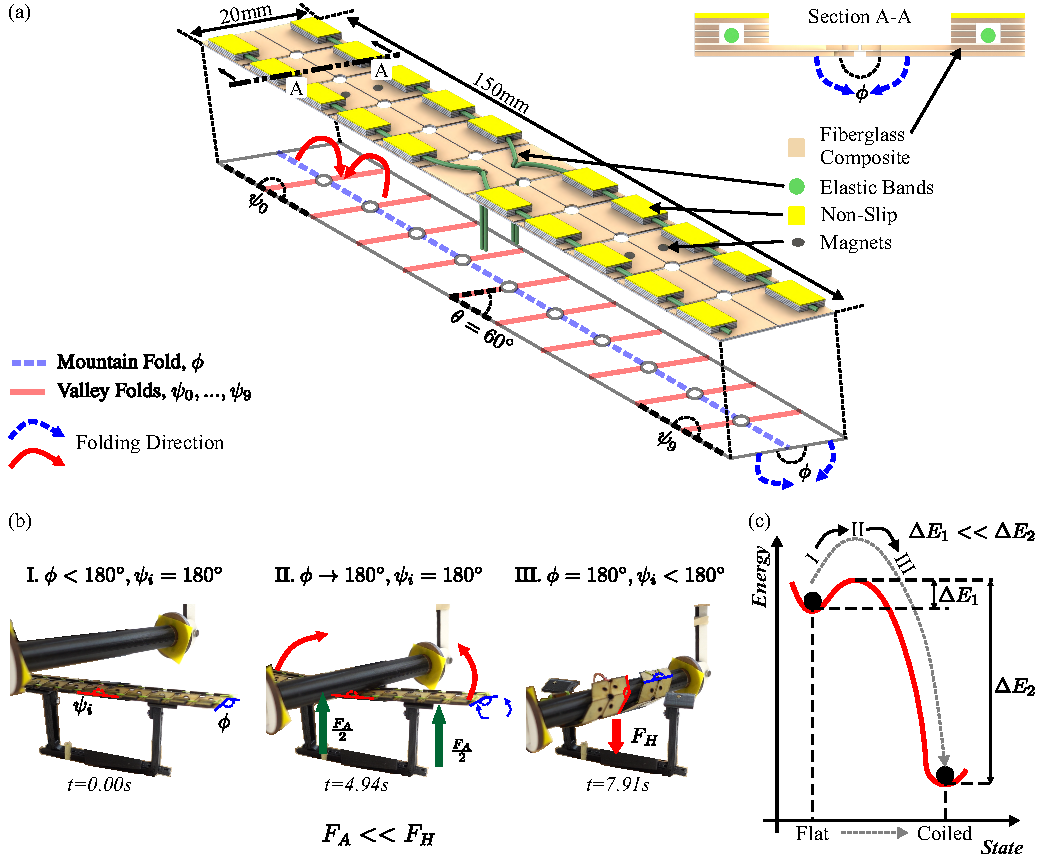
\includegraphics{figs/fig_2_design-intergration/Figure_2-corr-v2.pdf}
    \caption{Design and working principle of the bistable helical origami gripper. (a) 3D model of the gripper with schematic of the folding pattern and main components. The dashed blue line folds upwards, whereas the solid red lines folds down. These joints are unidirectional and, in conjunction with the pre-stretched rubber bands, allow for the bistable behavior. (b) State transition sequence. The gripper is pressed against a branch until the angle $\phi$ passes the horizontal, which is when the activation force, $F_A$ is overcome and the gripper is coiled. Once coiled, the gripper can only be removed with a force greater than the holding force, $F_H$, unless the tension in the elastic is released. (c) Energy states and transitions where the corresponding angles of $\phi$ and $\psi _i$ for each state can be seen in (b).}
    \label{fig:gripper_design}
\end{figure}

\subsection{Bistable Helical Origami Gripper}
\label{sec:bistable_origami_gripper}
Helical coiling is a widespread mechanism in nature for animals to grab objects with prehensile appendages or for plant tendrils to attach to objects. Coiling around an object has the benefit of increased contact area, and the ability to grasp differently sized objects in different orientations. These attributes confer several benefits when designing a gripper for attaching sensors to tree branches.
The increased surface area allows the gripper to provide more holding force, allowing for more payload and increased resistance to branch perturbations. Coiling also provides more robustness when coiling around branches with different diameters and compensating varying degrees of misalignment between the gripper and the branch.

Helical grippers are usually operated with pneumatic \cite{Kumar2018}, \cite{Hu2020}, \mbox{\cite{Pal2020ElasticMachines}}, hydraulic \cite{Galloway2016}, \cite{Hoang2020a}, cable-actuated \cite{Mazzolai2019}, magnetic \mbox{\cite{Wu2021StretchableTwisting}}, or electric systems \mbox{\cite{Meder2022AArrangement}}, \mbox{\cite{Shao2018BioinspiredActuators}}. However, actuators increase weight, complexity, and cost, making active helical grippers a sub-optimal solution for aerial delivery with MAVs, as well as scaling up the manufacture of the large number of devices potentially required for a dense sensor network. Therefore, a passively actuating gripper was developed, where the state transition for the bistable mechanism is triggered by contact with a branch, allowing the gripper to transition from an unfurled transport state to a coiled state around the branch. The gripper has been developed using an origami design method to minimize the number of mechanical components and facilitate manufacturing, while maintaining a high number of degrees of freedom to increase grasp strength and adaptability to branches with different grips and orientations. The guiding design principles are therefore: helical coiling allows for robust attachment to cylindrical structures such as branches, passive actuation and a bistable mechanism allows for coiling without the need for heavy and bulky actuators, and finally by utilizing origami manufacturing the structure can be made lightweight and easy to manufacture.

The proposed helical coiling gripper is an origami structure with multiple transversal folding joints (solid red lines, angles $\psi_i$, with $i \in \{0..9\}$, \textbf{Figure \ref{fig:gripper_design}a}) intersected by a single longitudinal folding joint (blue dashed line, angle $\phi$, Figure \ref{fig:gripper_design}a). The joints are manufactured to be uni-directional, such that each joint permits only folding towards one side of the gripper (i.e. $0\degree<\phi<180\degree$ and $0\degree<\psi_i<180\degree$ ). The folding directions are indicated with arrows corresponding to the fold lines. Two elastic bands (green in Figure \ref{fig:gripper_design}a) are arranged transversely, housed inside channels, and connected to the two ends of the gripper. They meet in the central segment and are routed through holes, passing through the gripper to the sensor box, where they are then tensioned around the hook (see \textbf{Figure \ref{fig:box}a}). These bands provide the necessary contractile force to enable the coiling of the gripper, and in conjunction with the pattern of uni-directional joints, confers a bistable behavior to the gripper. Additionally, a non-slip material (Dycem Non-slip), yellow in Figure \ref{fig:gripper_design}a is attached to the top of the fiberglass channels to increase the coefficient of friction with the substrate, thereby more than quadrupling the maximum holding force.

The gripper has two stable states: one unfurled state which is used for transport with $\phi<180\degree$ and $\psi_i=180\degree$ (Figure \ref{fig:gripper_design}b, Step I), and one coiled state for gripping with $\phi=180\degree$ and $\psi_i<180\degree$ (Figure \ref{fig:gripper_design}b, Step III). The unfurled state is reached by folding the gripper along the single longitudinal joint, whereas the coiled state is reached by folding the gripper along the multiple transversal joints.  A video of the bistable behavior can be seen in the Supplementary Video S1.

The state transition sequence is illustrated in Figure \ref{fig:gripper_design}b. In the initial step I, the gripper is unfurled. In this configuration, the gripper is folded along the longitudinal axis ($\phi < 180\degree$), and the continuity of the transversal joints over the longitudinal axis is broken, so they cannot be folded ($\psi_i = 180\degree$). Therefore, even if the pre-stretched rubber bands are producing a folding moment on the transversal folds, the gripper remains stable in the unfurled configuration. As illustrated in Step II, the transition is triggered by pushing the gripper against the branch, thus flattening the gripper until $\phi$ reaches $180\degree$. At this moment, the continuity of the transversal joints is restored, and the pre-stretched rubber bands cause the gripper to coil (Step III, $\psi_i < 180\degree$). The activation force $F_A$ required to trigger the state transition, and the holding force $F_H$ are characterized in the Section \ref{sec:characterization}.

The energy of the state transition is shown schematically in Figure \ref{fig:gripper_design}c. Starting from the initial unfurled stable state, a large change in the global energy state ($\Delta E_2$) can be induced by imparting a small amount of energy for the state transition ($\Delta E_1$), resulting in the second stable coiled state.
This behavior is desirable since the gripper should be easy to activate, yet once coiled around a branch it should remain firmly attached. The high compliance of the origami longitudinal joint reduces the necessary energy for the state transition ($\Delta E_1$), and the strength of the elastic band determines the overall gripping strength of the gripper, and thereby the energy of the second state ($\Delta E_2$). 
%Likewise, the activation  force required to trigger the state transition, $F_{A}$ is much less than the resulting holding force of the gripper, $F_{H}$ once the gripper is coiled.


\subsection{MAV Integration and Sensor Payload}
\label{sec:sensor_drone_integration}
As illustrated in Figure \ref{fig:box}c, to deploy the gripper, it is mounted on a off-the-shelf MAV (DJI Mavic Mini). The gripper is connected with small magnets to a U-shape holder mounted on the MAV. The connectors of the holder are angled such that $\phi$ is kept as 155\degree\ during transport, which is sufficient to prevent the state transition until contact with a branch.
Increasing this angle or decreasing the magnet strength would lower the activation energy, but $\phi$ must be chosen as a trade-off between ease of activation and resistance to perturbations during flight and accidental preemptive triggering. When the gripper is pressed against a branch, it begins to coil and self-releases from the magnetic latch. The sensor payload, including a battery, is encased in a 3D-printed box (37mm x 18mm x 23mm) with fiberglass lid, which is attached to the gripper via a string and the mechanism described in Section \ref{sec:retrieval}. The sensor payload consists of a TinyDunio with the Combo Sensor Tinyshield, which contains temperature, humidity, pressure sensors, and a 9-axis inertial measurement unit (IMU).
A fiberglass net was added to the top of the MAV, below the gripper, to protect the propellers from interference with foliage during the deployment.

\subsection{Retrieval Mechanism}
\label{sec:retrieval}
\begin{figure}[hbp]
    \centering
    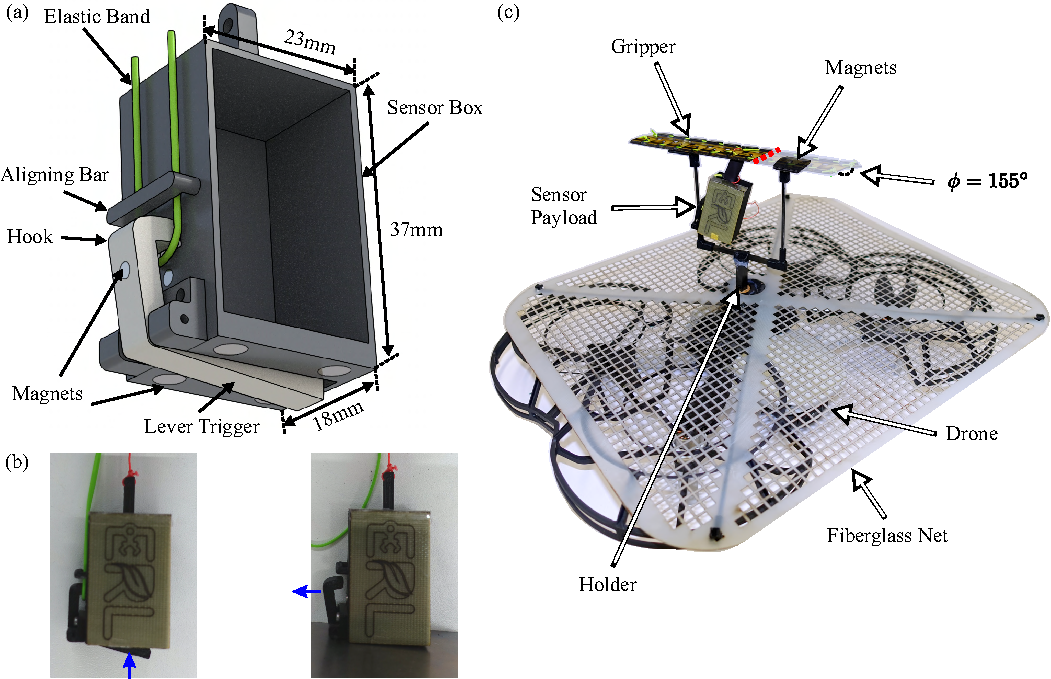
\includegraphics{figs/fig_8_box/Figure_8_box-corr-v2.pdf}
    \caption{Magnetic retrieval mechanism. (a) CAD view of the mechanism, when a metal plate approaches the bottom, the magnets pull it flush, the lever trigger is pressed and the hook releases the elastic. (b) Demonstration showing the release of the elastic when the lever is pressed; from the closed, tensioned configuration (left) to the open, released configuration (right). (c) Gripper in unfurled transport state on the MAV, with the different components labeled.}
    \label{fig:box}
\end{figure}
Once the gripper is coiled around a branch it should remain firmly attached. Simply pulling the gripper off will require the most force, having to counteract the entire contractile force of the elastic. To facilitate easy retrieval of the gripper, a magnetic latch was developed which releases the tension in the elastic band, thereby releasing the gripper from the branch. This mechanism can be seen in Figure \ref{fig:box}a. The basic functioning of the mechanism relies on the elastic bands (in green) tensioned around the hook (in beige) which can then be released by pushing the lever trigger. In order to tension the gripper, the elastic bands are routed through holes in each side of the gripper down to the box (see Figure \ref{fig:gripper_design}a), where they pass through the aligning bar before being attached to the hook. The aligning bar serves to keep the elastic from slipping too far on the hook and thereby remaining attached even though the lever trigger is pressed, since the travel of the lever is limited. Small magnets on the hook and box act to keep the lever hook in the closed position by default. When the gripper should be retrieved, a metal plate on the aerial robot is brought in contact with the bottom of the box. The four large 4 mm magnets on the bottom then pull the box flush with the plate, depressing the lever trigger, and anchoring it on the plate. Once the lever is depressed the elastic band is released and the gripper loses its contractile force, now attached only to the aerial robot. Figure \ref{fig:box}b shows the mechanism  functioning, where the lever trigger is activated by a metal plate, thereby releasing the elastic. The collection process of the gripper also can be seen in Supplementary Video S2, where it possible to observe the green elastic being released, and the gripper then collected.

\subsection{Geometric Characterization}
\label{subsec:parameter_selection}
Functional attributes of the gripper such as the minimum and maximum graspable diameters ($D_{min}$ and $D_{max}$ respectively) and the coiled length ($C$) depend on the selection of design parameters. There are four main design parameters (see \textbf{Figure \ref{fig:parameters}}): $L$, the end-to-end length of the gripper, $w$, the width of the gripper, $\theta$, the slant angle of the gripper, and $n$, the number of segments. The effect on the functional attributes of the different design parameters as well as the reasoning for their choice are explained here. 

\begin{figure}[hbp]
    \centering
    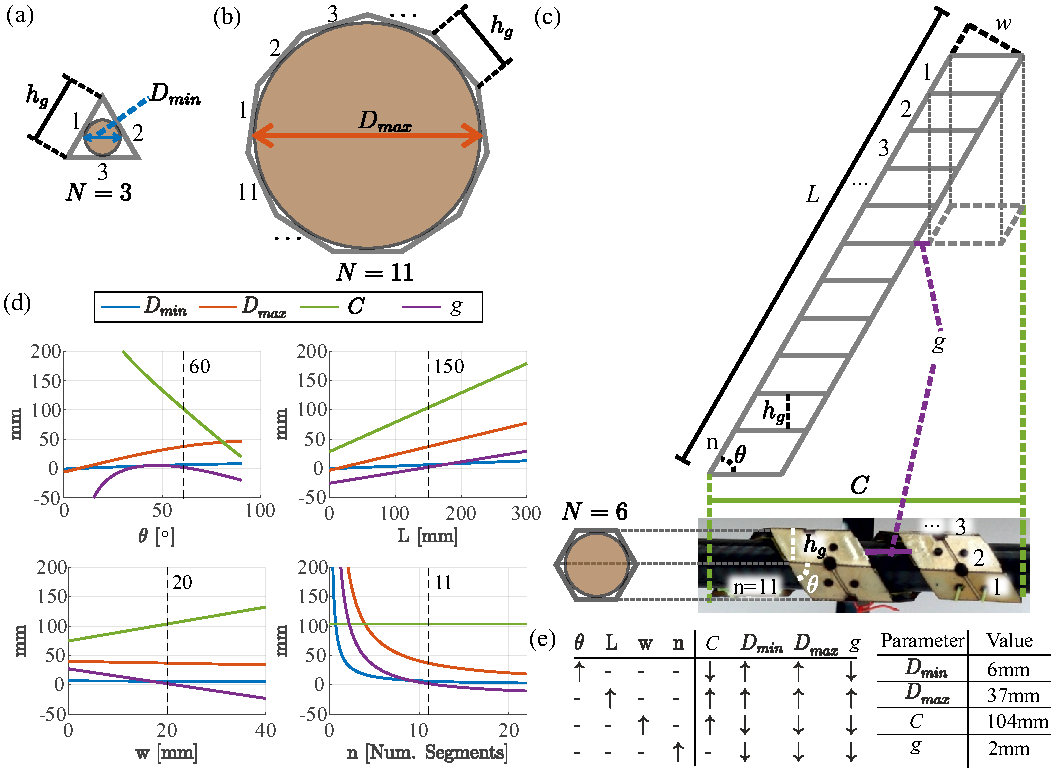
\includegraphics{figs/fig_7_design_parameters/fig_7_design_parameters_gap_v2-corr-v2.pdf}
    \caption{Geometric design parameters of the gripper. (a) The minimum diameter  $D_{min}$, with $N=3$ (b) Maximum graspable diameter $D_{max}$ of the gripper where $N=n=11$, the number of segments of the gripper. (c) Parameters of the gripper and their effect on the coiled length $C$. (d) Plots showing the effects of increasing each of the gripper parameters in turn on the attributes, chosen values are shown as dashed vertical lines. (e) (Left) Table showing the effect of increasing each of the parameters $\theta, L, w, n$ on the gripper attributes coiled length $C$, the minimum and maximum diameters ($D_{min}$ and $D_{max}$ respectively), and the gap, $g$. (Right) Gripper attributes for our chosen values.}
    \label{fig:parameters}
\end{figure}

The cross section of a branch with the gripper coiled around it  can be represented as a circle inscribed in a regular polygon, where the circle is the branch and each edge of the polygon represents the height of one segment of the gripper, $h_g$  (see Figure \ref{fig:parameters}a, b, c). Note that the edge length of the polygons, $h_g$, is the same for both the minimum and maximum diameters in Figure \ref{fig:parameters}a and \ref{fig:parameters}b. The $N$ denotes the number of edges of polygon in the cross-section when coiling.

The maximum diameter, $D_{max}$ (Figure \ref{fig:parameters}a), is one full coil around the branch with no overlap of the segments, so the full length of the gripper, or $N=n$ (which for our chosen parameters is $N=11$). In other words, the number of sides of the polygon is equal to the number of segments of the gripper. The smallest coil fully encircling a branch is a triangle, where the number of sides of the polygon, $N=3$. This is the theoretical minimum. Due to collision constraints from the channels, when folding in practice the smallest achievable configuration is more like a square, with $N=4$.
The minimum and maximum graspable diameters can therefore be constructed as follows (see the Supplementary Section A and Supplementary \textbf{Figure S1} for derivation):

\begin{equation}
    D = \frac{\sin \theta}{n \tan \frac{\pi}{N}} \left( L - \frac{w}{\tan \theta}\right)
    \label{eq:diameter}
\end{equation}
with $N=n$ for $D_{max}$, and $N=3$ for $D_{min}$.

The horizontal coiled length of the gripper on the branch, $C$, (Figure \ref{fig:parameters}c), is given geometrically by the following equation (see the Supplementary Section A and Supplementary Figure S1 for derivation):
\begin{equation}
    C = w\left( \frac{1+\cos^2 \theta}{\sin \theta} \right) + L\cos \theta
    \label{eq:coiled_length}
\end{equation}

Note that the coiled length, $C$ is independent of the state of folding of the gripper, it is the same regardless of whether the gripper is unfurled (Figure \ref{fig:parameters}c top) or coiled around a branch of any diameter (Figure \ref{fig:parameters}c bottom). It depends solely on the parameters $w,L,$ and $\theta$. 

Once coiled there is a gap, $g$, between the coils dependent on the diameter gripped and gripper parameters. Depending on the chosen parameters, there could also be an overlap instead of a gap between the segments. This value is given by (see the Supplementary Section A and Supplementary \textbf{Figure S2} for derivation):

\begin{equation}
    g = \frac{N \cos \theta}{n}\left(L - \frac{w}{\tan \theta}\right) - \frac{w}{\sin \theta}
    \label{eq:gap}
\end{equation}

where negative values denote an overlap of the segments as opposed to a gap. An overlap is generally undesirable as it would cause the segments to collide when coiling, either preventing successful coiling completely or reducing the segments in contact with the branch, instead causing coiling on top of the previous coil.

The effect of increasing each of the design parameters ($L, w, \theta,$ and $n$) in turn on the functional attributes of the gripper can be seen in Figure \ref{fig:parameters}d and e. The values of the attributes for the chosen design parameters are also shown in the table on the right in Figure \ref{fig:parameters}e.

The design parameters were selected considering several functional requirements and constraints. We started by selecting the length of the gripper $L$. 
The longer the length of the gripper, the larger the diameter of the branch that can be coiled. At the same time, because the gripper is transported in the unfurled state on the MAV, long grippers are more likely to become entangled in vegetation and can be challenging to transport with smaller MAVs. Therefore, we decided to limit the length of the gripper to 150 mm.

The angle $\theta$ between the transversal joints, seen in Figure \ref{fig:gripper_design}a, determines the degree of helicality of coiling. At 90\degree\ the strip simply coils perpendicular to the joint, with no lateral coverage, whereas smaller angles of $\theta$ result in more helical coiling, with a larger coiled length, $C$. Perpendicular coiling with $\theta=90\degree$ constitutes complete overlap and is therefore undesirable. 
Increased  coiled length, $C$, results in increased contact area with the branch, and is therefore desired to be maximized. The gap between the coils $g$ should be minimized such that for the smallest configuration two neighboring coils are close but not overlapping. To decrease $g$, the value of $\theta$ should be large, but increasing it too much reduces the minimum diameter graspable, as well as decreasing $C$. A value of $\theta=60\degree$ was chosen. The trade-off between these values can be seen in the top left graph of Figure \ref{fig:parameters}d.

Once $L$ and $\theta$ are selected, we considered $w$. Both $w$ and $\theta$ influence gap width, and since overlap is undesirable, $w$ can be computed from Equation \ref{eq:gap} for $g=0$. For the chosen parameters this equals $w=20 mm$, with a slight safety margin.

With fixed $L, \theta$ and $w$, the number of segments $n$, affects $D_{min}$, $D_{max}$ and $g$. Decreasing the number of segments increases the segment height, $h_g$,  which increases the minimum and maximum graspable diameters, and the gap, $g$, between coils. Too few segments make $h_g$ too large and smaller branches ungraspable. Too many segments make routing the elastic difficult since a channel is required for each segment. Additionally, it is desired to be odd such that there is a segment in the middle, and when coiled which provides an attachment point at the bottom for the sensor. The value chosen is 11. 

The vertical dashed lines in the plots of Figure \ref{fig:parameters}d show the chosen values, which show the tradeoff between maximizing $D_{max}$ and $C$, and minimizing $D_{min}$ and $g$.

Using Equation \ref{eq:diameter} for the given dimensions of the gripper this results in a graspable range of diameters between 6 mm (11 mm for $N=4$) and 37 mm. Therefore for the experiments branches between 8 mm and 38 mm were chosen.


\subsection{Experimental Characterization} % experimental characterization
\label{sec:characterization}
In order to characterize the gripper, the activation force, number of successful activations with different tilt and rotation offsets, and maximum holding force for different branches were empirically determined. 

\subsubsection{Activation Force}

\begin{figure} [htpb]
    \centering
    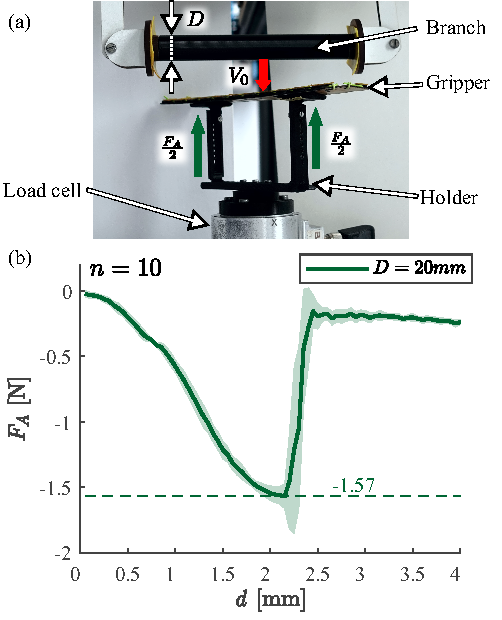
\includegraphics{figs/fig_3_activation_force/Figure_3.pdf}
    \caption{Activation force measurements. (a) Test setup for measuring the activation force, $F_A$, the force needed to transition between the unfurled and coiled states. The gripper is mounted on the holder which is attached to the load cell, the branch then moves down at a fixed speed and pushes down on the gripper until it is activated. (b) The force curve of the activation energy as a function of the displacement of the branch (mm), 1.57 N are needed to activate the gripper. The curve shows the mean and standard deviation (dark and light green) from ten trials.}
    \label{fig:activation_force}
\end{figure}

An important consideration for the practical use of the gripper is the force required to transition between the states, since the MAV must be able to produce this activation force during flight to successfully coil the gripper around a branch. To this end, the activation force of the gripper is measured. For these tests, the gripper is mounted on its magnetic holders, which are connected to a load cell measuring the imparted force on the holder, see \textbf{Figure \ref{fig:activation_force}a}. A 3D printed ABS cylinder representing a branch is lowered at a constant 5 mm/s until the gripper is engaged. The resulting force can be seen in Figure \ref{fig:activation_force}b as a function of the displacement, $d$, of the branch. The force steadily increases as the test branch pushes down on the gripper, until the activation threshold angle is overcome, the gripper is coiled and the applied force is zero. Here, the activation force required is 1.57 N, which is significantly lower than the maximum thrust that the MAV can produce, and the entire activation sequence takes around 400ms, even with the relatively slow  branch movement.

\subsubsection{Robustness to Tilt and Rotation Offsets}
In this section we investigate the deployment of the gripper on branches of different diameters, and consider both angular and translational offsets, which could result from the inclination of the branch and from misalignment of the gripper and branch caused by errors or drift when commanding the MAV.

\begin{figure} [htbp]
    \centering
    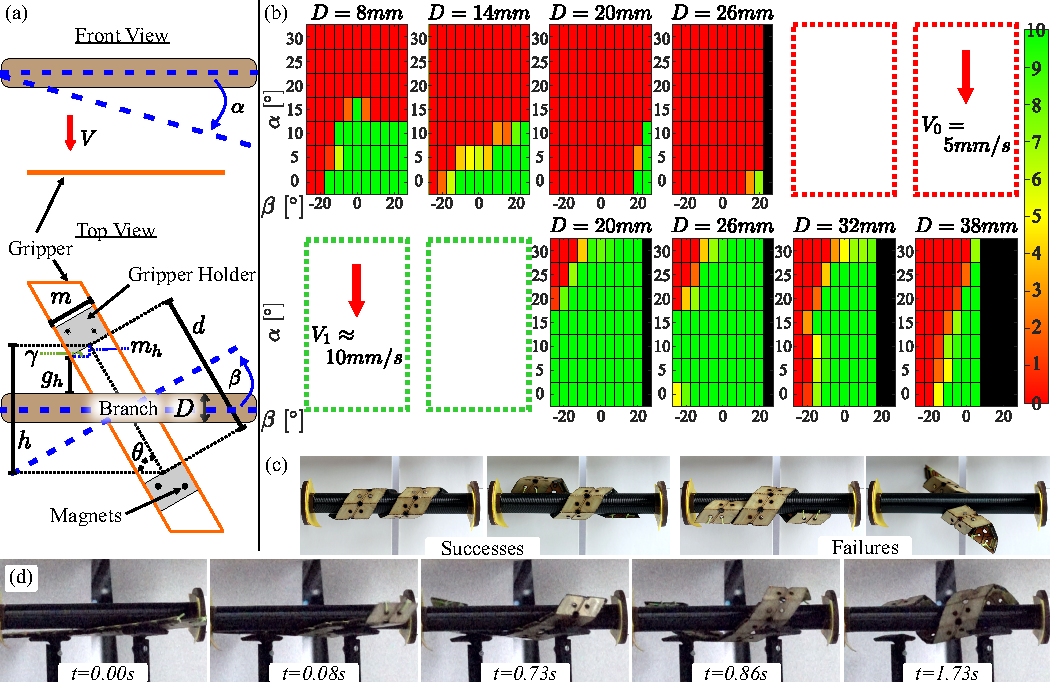
\includegraphics{figs/fig_4_successful_activation/Figure_4-corr.pdf}
    \caption{Resistance to tilt and rotation offsets. (a) Front and top view of the experimental test setup for low velocity and high velocity experiments ,with the gripper (orange) approaching a branch (brown). The gap from the branch to the gripper holders (gray) depends on the branch diameter $D$, and distance between the holders $d$. Both the branch tilt angle $\alpha$ and the rotation of the gripper $\beta$ can be modified.  (b) Number of successful activations for different branch diameters and tilt and rotation offsets. The top row are low velocity experiments, the second row are high velocity experiments. The scale from red (0) to green (10) demonstrates the number of successful activations out of 10. Black cells show unreachable configurations due to physical limits of the test setup when combined with different branch diameters. The dashed red lines denote experiments which were not conducted since they would have all failed, and dashed green lines represent experiments which were not conducted since they would have all succeeded. (c) Sample configurations of successes and failures. At least one full coil of the gripper must be coiled on the branch to be considered a success. (d) High-speed capture of the gripper coiling, low velocity experiment.}
    \label{fig:number_successful_activations}
\end{figure}

For these experiments we used a setup similar to the previous one (Figure \ref{fig:activation_force}, without the load cell), but with the addition of controllable tilt ($\alpha$) and rotation ($\beta$) offsets (\textbf{Figure \ref{fig:number_successful_activations}a}). A tilt angle of zero means that the branch
is horizontal (when viewed from the front). A zero rotation angle is with the gripper rotated \mbox{30\degree\ } from the vertical (viewed from the top), i.e. such that the transverse cuts are parallel with the branch. We tested two vertical speeds (5 and 10  mm/s) to simulate a slow and more dynamic attachment of the sensor to the branch ($V$ in Figure \ref{fig:number_successful_activations}a with $V_0=5mm/s$ for the low velocity, and $V_1=10mm/s$ for the high velocity), and branch diameter $D$ ranging between 8 mm and 38 mm, with 6 mm increments. The results of these experiments can be seen in Figure \ref{fig:number_successful_activations}b. The color in each cell represents 10 trials for one combination of tilt and rotation angle. The color is on a scale from 10 successful activations (green) to none (red). A test is considered a success if there is at least one full coil around the branch, see Figure \ref{fig:number_successful_activations}c. Black signifies unreachable configurations with the test setup, particularly applicable with larger branch diameters. For instance, using the 38 mm branch with angles of $\beta$ larger than 10\degree\ would result in collision of the branch with the holders when engaging, since the inner distance between the centers of the gripper holders is only 75 mm (a more detailed discussion on this follows later with the translational offset, see \mbox{\textbf{Figure \ref{fig:number_successful_activations}a}}). Due to the large number of possible tilt and rotation angle combinations for each branch diameter with repetitions ($7\cdot 11\cdot 6\cdot 10=4620$ tests) exhaustive testing of all cells is performed only until the ``limit''angles are found. For instance, if no successful activations are achieved with a particular tilt angle, steeper tilt angles are not tested since they would merely perform worse, these are then listed as failures. Similarly for rotation angles, since the gripper only fails with extremes and not for intermediate angles, only these limits are tested, with the centers then filled in as successes. This also applies to branch diameters, since larger branch diameters are more challenging to grasp, and smaller ones are easier, once almost all tests fail or succeed further tests were not conducted (see dashed red or green lines in Figure \ref{fig:number_successful_activations}b).
%add comment that faster speeds are better for coiling (revision1), quasi dynamic tests

With a speed of 5 mm/s the gripper manages to successfully engage on the smallest two diameters, with performance degrading quickly on larger diameters. Larger tilt and rotation offsets also reduce performance. During these tests the vertical movement occurred with a speed of 5 mm/s, which is quite slow when compared with the activation of the gripper (400ms when activated with a speed of 5 mm/s). For the larger branches the gripper was already coiling at the ends before they could reach around the branch, and therefore before they are able to engage for coiling. A speed of 10 mm/s allows for a more dynamic engagement and the gripper can successfully attach to the full range of diameters tested, with performance again degrading with increasing branch diameter and larger tilt and rotation offsets. During high velocity engagement, the inertia of the contact along with the branch quickly passing the gripper holders facilitates coiling for larger branches by enabling the end of the gripper to reach the top of the branch before they finish coiling. A further increase in speed could also increase the probability of successful coiling. However, we expect an upper limit due to the increased risk of collision of the MAV with the branch and potential gripper tear due to the high speed collision.

These results show that the gripper is able to successfully attach to branches varying in diameter between 8 to 36 mm, with the number of successful activations decreasing with larger branch diameters. Larger tilt and rotation offsets also negatively affect performance. Interestingly, in all cases, the best performance is not achieved with a rotation angle, $\beta=0$, as expected, but for larger positive rotations. In this case, the gripper is becoming more and more perpendicular with the branch. In this scenario, larger branches are easier to grasp since the ends of the gripper are further apart and it is more likely to successfully be able to encircle the branch, even if the folds are not perfectly aligned to be parallel with the branch. This suggests that the adjusting the mounting angle of the gripper on the MAV to have a larger $\beta$ angle would increase the chance of success. These results could also be used to optimize the design of the gripper by decreasing $\theta$, resulting in a longer coiled length, $C$, and changing the mounting angle to still have successful activation. The increase in holding force would have to be experimentally verified.

These tests also allow for an impression for the robustness of the origami joints of the gripper, since one gripper lasted for more than 2000 tests (coiling and uncoiling) before a joint broke. A tear on the edge of the Kapton joint will propagate until eventually the entire joint is broken, leading to premature failure, but when care is taken to avoid this during manufacturing the joints are quite robust.

Translational offsets parallel to the branch will have no impact on the coiling behaviour since the contact point on the gripper remains the same. Axial misalignment or translational offsets perpendicular to the branch can be split into two cases: contact between the holders, and outside. For contact outside the holders the coiling will fail. It is expected that when the contact occurs between the holders, increased distance from the center increases the activation force and chance of failure. In practice, however, when contact occurs inside the holders coiling will succeed, and the offset is not relevant. This is shown in Figure \mbox{\ref{fig:number_successful_activations}a}. Since the holders are oriented such that the transversal joints on the gripper are perpendicular to the branch, the effective distance between them, $h$ is given by $h=d \sin \theta$, where $d$ is the distance between the holders. The distance between the branch and one of the holders, $g_h$ for a branch of diameter $D$ is given by $g_h = (h-D-2m_h)/2$. Where $m_h$, the distance from the center of the holder to the edge, is $m_h = m \sin \gamma$ for a holder with a width of $m$, and with $\gamma= 90\degree - \theta$. In our case the distance between the holders is 75 mm, and therefore $g_{h, min}=23.45 mm$ and $g_{h, max}=8.45mm$ for the minimum and maximum branch diameters (8 mm, 38 mm), respectively. These distances are sufficiently small that translational offsets perpendicular to the branch do not have an appreciable effect on the success of coiling, either the branch is within the holders and coiling is successful, or not.


\subsubsection{Maximum Holding Force}

\begin{figure} [htbp]
\centering
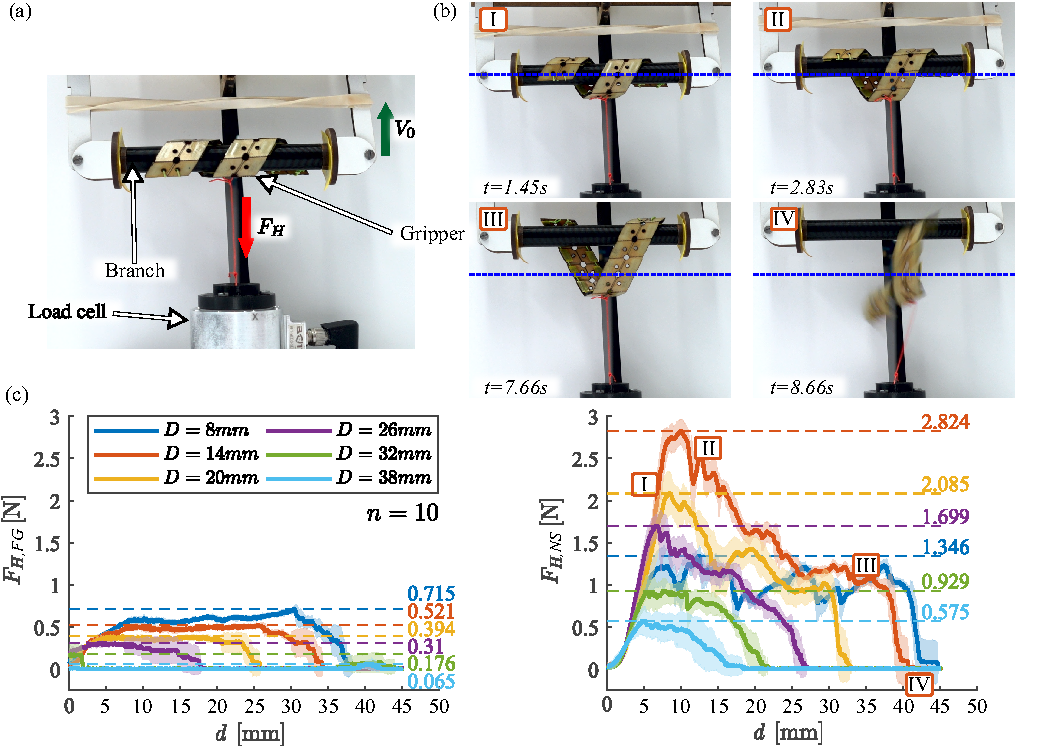
\includegraphics{figs/fig_5_holding_force/Figure_5-corr.pdf}
\caption{Holding force measurements. (a) Test setup for measuring $F_H$, the holding force until the gripper is pulled from the branch. The branch is moved upwards at $V_0$, with the load cell attached to the gripper measuring the resulting force. (b) Snapshots at different times during the 14 mm diameter branch test with non-slip.  Larger branch diameters result in lower attainable forces, with the exception of the 8 mm branch with non-slip material, since the branch was too small for the gripper to be able to properly encircle it. (c) Curves showing the holding force for the gripper with just fiberglass ($F_{H, FG}$, left), and with non-slip material ($F_{H,NS}$, right). Measurements were repeated ten times ($n=10$).}
\label{fig:maximum_holding_force}
\end{figure}

The strength with which the gripper can hold onto branches, the maximum holding force, determines not only the maximum payload, but also resistance to disturbances such as wind. The more weight that the gripper is able to hold, the larger the payload capacity and the more flexibility the solution has with regards to sensor selection.
In these tests, a string connects the gripper to a load cell. The gripper is then attached to the branch, which is moved up at 5 mm/s until the gripper has disengaged from the branch. This testing setup can be seen in \textbf{Figure \ref{fig:maximum_holding_force}a}.
%value is a lower bound since pulling on central coil is worse case scenario (compared with pulling one of the ends)
Results can be seen in {Figure \ref{fig:maximum_holding_force}c}, where tests are conducted ten times per branch diameter $D$ for regular fiberglass ($F_{
H,FG}$) shown in the left graph, and also with a high friction non-slip layer attached ($F_{H, NS}$), in the right graph. The solid line is the mean of these tests and the lighter area is the standard deviation, tests were conducted 10 times per scenario. Figure \ref{fig:maximum_holding_force}b shows the different stages of unfurling when the gripper is pulled from the center, the corresponding holding forces for each of the timesteps are labeled in Figure \ref{fig:maximum_holding_force}c.
The left graph in Figure \ref{fig:maximum_holding_force}c demonstrates the maximum holding force achievable with the basic gripper, with the contact between fiberglass and the ABS of the cylinders acting as stand-ins for branches. ABS is much smoother than organic tree branches, the actual values obtainable outside on rougher branches are therefore likely much higher than the conservative values measured here. Since the friction between the gripper and substrate plays an important role for the maximum holding force, a high friction non-slip material (Dycem Non-slip) was attached to the fiberglass channels which contact the branch, these results can be seen in the right graph in Figure \ref{fig:maximum_holding_force}c. They are significantly higher, more than quadrupling the holding force when compared with just the base fiberglass.
Since the holding force depends on the number of coils the gripper has around the branch, it is also dependent on the size of the branch it is attaching to. Similar to the number of successful activations, the trend for the maximum holding force is that it decreases for increasing branch diameter. With larger branch diameters the gripper is more unfurled and able to encircle the branch with fewer coils, and therefore the holding force is decreased. This trend holds true for all plots except the 8 mm branch with non-slip material, marked in black. This is an outlier since the diameter of the branch is almost smaller than the minimum inner diameter of the gripper, resulting in a lack of compressive force, and thereby the gripper is able to exert less friction, hence holding force (see also Section \ref{subsec:parameter_selection}, where the minimum graspable diameter is discussed, here $N=4$, not 3 due to the channels for the elastic).

\subsection{Preliminary Field Tests}

To perform preliminary field tests, the gripper and sensory payload are integrated with the MAV as described in Section \ref{sec:sensor_drone_integration}. The deployment process is shown in \textbf{Figure \ref{fig:outdoor_activation}}. A video of the outdoor gripper deployment and collection can be found in Supplementary Video S2.  First, the MAV is aligned with the branch. It is sufficient to align the MAV to be perpendicular with the branch since the gripper holder on the MAV is already placed at 30\degree, which, when combined with the 60\degree\ cut angles on the gripper, allows the cut lines to be parallel with the branches. This configuration allows the gripper to coil well on the branch and simplifies piloting. Once aligned, the MAV is positioned roughly 10 cm below the branch, then moved rapidly upwards (Figure \ref{fig:outdoor_activation}a). Larger distances would facilitate coiling of the gripper as long as the impact does not destabilize the MAV. This dynamic movement of the robot allows the gripper to deploy onto the branch. Once the gripper has coiled around the branch, the sensor payload is also attached, and thus deployed (Figure \ref{fig:outdoor_activation}b).

Once attached to the branch, the sensors record and transmit environmental data to a cloud over Wi-Fi, allowing real-time monitoring on a smartphone. Figure \ref{fig:outdoor_activation}e shows the interface of the web-widget displaying the current streamed values. Sample temperature, humidity, pressure, and light intensity values collected from a deployed sensor can be seen in Figure \ref{fig:outdoor_activation}f.

Once the sensor has completed its measurement cycle, it must be collected to retrieve the sensor and data (Figure \ref{fig:outdoor_activation}c). To this end, the retrieval mechanism (Figure \ref{fig:box}a) was incorporated into the payload box. This allows a ferromagnetic plate on the MAV to attach to the box, and release the tension in the gripper, thereby releasing it from the branch and leaving it anchored to the plate and the MAV (Figure \ref{fig:outdoor_activation}d). The MAV can then land and the collected sensor and data can be retrieved.

\begin{figure} [htbp]
    \centering
    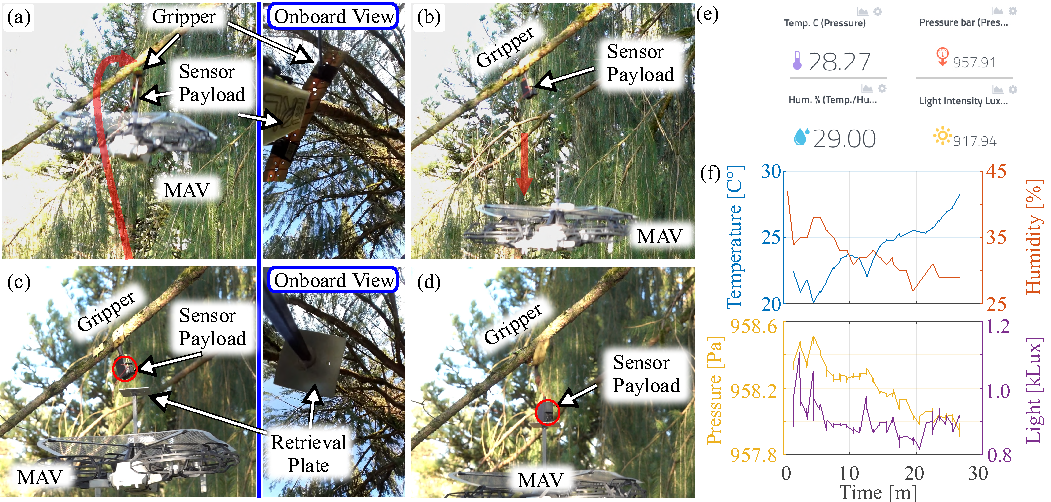
\includegraphics{figs/fig_6_outdoor_deployment/Figure_6-corr-v2.pdf}
    \caption{Outdoor gripper deployment. (a) (Left) The MAV approaching the deployment site with mounted gripper and sensor. (Right) Up-ward facing camera view from onboard the MAV. (b) Activating the state transition of the gripper and deploying the sensor. (c) (Left) Successfully deployed gripper with attached sensor payload, the MAV returns. (Right) Up-ward facing camera view from onboard the MAV. (d) Collection of sensor and gripper with retrieval plate mounted on the MAV, note the release in tension of the green elastic  between (c) and (d) (red circle). (e), (f) sample measurements and logs taken with the sensor.}
    \label{fig:outdoor_activation}
\end{figure}


\section{Conclusion} %& discussion
In this paper, the design, characterization, and testing of a bistable helical gripper made with origami manufacturing was presented. When compared with existing solutions to deliver sensors, our method allows for the attachment to small branches located on the outer canopy, whereas previous approaches focused on the main trunk and large branches. Our gripper demonstrates successful attachment to branches with diameters of 8 to 38 mm, as determined by the geometric parameters chosen. Moreover, depending on the thickness of the branch, the gripper managed to successfully attach with angle offsets of -20\degree to 20\degree, and with a branch tilt offset of up to 30\degree. With a high friction non-slip material on the gripper, the maximum attained holding force was 2.8 N, which allows the gripper to hold more than 56x its own weight (5 g).

While origami fabrication is scalable, grasping smaller or larger branches presents additional challenges. Some very small branches may not be stiff enough to induce a state transition when the aerial robot initiates contact. This problem can be solved by integrating actuators into the gripper, at the expense of a more complex and heavier design. Grasping larger branches requires longer grippers, which can more easily become entangled in vegetation during flight. One solution is to increase the complexity of the folding pattern to avoid carrying the gripper in the unfurled state.

Future developments will focus on improvements in both the delivery strategy and the origami gripper. The MAV used in the field tests was flown manually, and alignment between the branch and MAV was also done manually. Misalignment between the gripper and branch was the largest source of error leading to attachment failure. Since the deployment and retrieval maneuvers can be challenging to perform in dense forest environments, increased automation in the deployment pipeline would increase robustness and reliability. A first step would be to automatically align with the branch using a camera and visual servoing approach. Next, the distance to the branch would be adjusted based on the output of a depth sensor. Finally, once the MAV is 10cm below the branch the deployment sequence will be initiated where the MAV moves rapidly upwards to attach the gripper, stabilizes after the impact and returns. Mounting the gripper on an orientable holder would yield different applications, for instance, vertical attachment for data collection of growing plant stalks. Here the adaptable origami gripper would expand with the growing plant and not require manual re-sizing, extending the scope of the gripper thanks to the versatility of origami manufacturing. By incorporating a flex sensor to measure the curvature of the gripper the diameter of the branch could also be measured and monitored, acting as a dendrometer in previously inaccessible locations. Using the IMU to measure the oscillations of the branch could provide an estimate of the wind speed in dense tree crowns where the actual wind speed could not be measured. Incorporating biodegradable layers into the gripper could allow it to automatically drop off the branch and fall to the forest floor after a defined time, allowing the sensor to be simply collected from the ground.
Finally, although the gripper was tested to deploy sensors on branches, it could be applied in any scenario where sensors need to be attached to cylindrical objects, such as for inspection and monitoring of pipes or power lines in industrial settings. 

% Experimental section
\section{Experimental Section}

\threesubsection{Origami Manufacturing}\\
The origami was manufactured using sheets of 0.3 mm FR-4-HF fiberglass with DuPont$\textsuperscript{TM}$ Pyralux $\textsuperscript{\textregistered}$ LF Bond Ply LF0111 with 0.1 mm thickness as both a Kapton layer and adhesive. Each layer was cut with a CO2 laser (Trotec 360 Speedy). The layers were then stacked and bonded in a Fontjine LabManual 300 hydraulic heat press. Pressure, temperature, and time settings were chosen to comply with curing settings given by the adhesive sheet manufacturer. A regular origami composite consists of a bottom layer of fiberglass, the Kapton and adhesive layer, followed by another top layer of fiberglass (See Supplementary Section C for a list af all the different layers). The unidirectional joints described in Section \ref{sec:bistable_origami_gripper} were manufactured by cutting the pattern on the side that is intended to fold, and engraving the same pattern on the other side, which prevents folding in that direction. Since some sections of the gripper have cuts on all sides, extra supports are added to align these sections and hold them in place  during manufacturing. These are removed by a laser release cut, after bonding, before the gripper is assembled. After the supports are removed, the uni-directional folds must enabled, this involves snapping the fiberglass along the engraved lines, thus "breaking" the joint and allowing the joint to move freely in the direction opposite the engraving.

To ensure uniform distribution of the contractile force of the elastic elements over all segments of the gripper, special channels are manufactured. If the band was simply routed through holes cut in the gripper, friction between the band and the outline of the holes would prevent the band from exerting a uniform force over all elements. The elastic band used is Autain Zim Fluo 1.6 kg silicone band with a diameter of 0.9 mm. When tensioning the gripper the elastic was stretched to 150\% of its original length to provide the contractile force. The channels are 1.2 mm thick to allow the elastic band through. Manufacturing these channels requires an additional bonding step since the channel elements cannot be bonded concurrently with the main gripper, due to the height difference between the top of the channel and the top of the gripper. The pressure differential would prevent proper bonding of the adhesive on the gripper since only the top of the channels would be pressed. Therefore, first the gripper and channels with supports are cut and bonded separately. Then, the two parts are bonded together. See Supplementary Section C for more information.

To increase friction between the gripper and substrate Dycem Non-slip high friction material is added to the top of the channels. The laser-cut pieces are manually attached with cyanoacrylate after the gripper has been manufactured. 


\threesubsection{Experimental Setup}\\
All force measurements were conducted with a Bota Systems Medusa 6 axis Force/Torque sensor. 
Due to the initial non-zero measurement of the load cell, the first 100 data points without load were averaged and subtracted from all subsequent measurements to zero the measurements. Additionally, unless otherwise specified, all force measurements were conducted 10 times, and the mean and standard deviation plotted. The different test setups are shown in the respective Figures \ref{fig:activation_force}, \ref{fig:number_successful_activations}, \ref{fig:maximum_holding_force}. These consist mainly of the low velocity setup, with substitution of either load cell, or the rotation and tilt mechanisms; and the high velocity setup. The low velocity setup has a constant 5 mm/s vertical movement generated by rigidly connecting the test setup with a 3D printer, with the moving branch connected and controlled with the printer's movable Z-axis. The high velocity test is similar, consisting of the tilt and rotation mechanisms, but with the movable branch connected to a guide rail which allows it slide freely, and be dropped, vertically. The branch is first raised a fixed distance, 1 cm, and then dropped to result in a speed of around 10 mm/s, to simulate the speed of the MAV as it accelerates upwards to engage the gripper. This is more than twice the previous speed, but still well within speeds that the MAV can generate. The drop speed of the high velocity setup was measured by counting frames of a high-frame rate camera. In both the low velocity and high velocity cases, by tilting the branch or rotating the gripper assembly different tilt and rotation offsets can be simulated.\\
%  Describe test setup and testing methodology, inc. load cell, data cleaning etc.\\
\threesubsection{Outdoor Tests}\\
For outdoor tests the gripper was mounted on commercially available MAVs, with additional protection against foliage. The MAV shown here is the DJI Mavic Mini. See the Supplementary Section C, Supplementary \textbf{Figure S4}, and the Supplementary Video S3 for the integration with the DJI/Ryze Tech Tello MAV. In addition to the included propeller guards to protect from lateral collisions, a fiberglass net was added to the top of the MAV, below the gripper, to protect the propellers from interference with foliage during the deployment. The fiberglass net was created by laser cutting a lattice of 4 mm squares in a fiberglass sheet with 0.2 mm thickness. To attach this to the MAV, mating parts were 3D printed and the net was supported with 2mm hollow carbon rods. The sensor system used is based on the TinyDuino platform, with a separate 3.7 V 150 mAh LiPo battery for power. The Combo Sensor Tinyshield was used, with temperature, humidity (Silicon Labs Si7020-A10), barometric pressure (Bosch BMP280), 9-axis IMU (ST LSM9DS1), and ambient light (TAOS TSL2572).
The contribution of the different components to the total take-off weight is shown in Table \ref{tab:weight}. The gripper weighs less that 5 grams, without the no-slip material. 

\begin{table}
    \centering
    \caption{Weight of different components. The take-off weight is 352.20 g, and the assembly deployed on the branch weighs 19.98 g, with the gripper weighing less than 5 g.}
    % \begin{tabular}{c|c|c}
      \begin{tabular}[htbp]{@{}lrr@{}}
          & Mass(g) & \% Total Mass \\
        \hline
        MAV & 148.88 & 42.3 \\ 
        Battery & 96.65 & 27.4\\
        Lateral Propeller Guards (Commercial) & 47.56 & 13.5\\ 
        Top Propeller Net and Gripper Holder (Custom) & 39.13 & 11.1\\
        Sensors (incl. battery) & 8.55 & 2.4\\
        Sensor Box (excl. Sensors) & 6.45 & 1.8\\
        Gripper & 4.98 & 1.4\\
        \hline
        Total & 352.20 & 100
        
    \end{tabular}
    \label{tab:weight}
\end{table}
Preliminary outdoor tests were conducted during several different testing runs, and with different trees (See Supplementary Video S2, S3). To facilitate easy retrieval in case of failure, branches accessible from the ground were chosen.


\medskip
\textbf{Supporting Information} \par %Please delete the Supporting Information statement if it is not applicable. Please supply Supporting Information in another file. Supporting information should not be provided in .tex format
Supporting Information is available from the Wiley Online Library or from the author.



% Acknowledgements
\medskip
\textbf{Acknowledgements} \par %delete if not applicable))
This work was supported by the Swiss National Science Foundation through the Eccellenza under Grant number 186865. The authors thank Carlos Augusto Guija Deza for help with the retrieval mechanism.

% References
\medskip

% Use the following code if you wish to generate your bibliography with BibTeX;
% replace the string "MSP-template" below with the name(s) of
% the BibTeX data base(s) you want to use.
% The resulting bibliography-output (the content of the .bbl file)
% must be pasted back into this file before submission.
% Please also include your BibTeX data base file(s) in your submission
% so that we can re-run BibTeX if necessary.
%
% \bibliographystyle{MSP}
%\bibliography{MSP-template}
%\bibliography{references.bib}


% \begin{thebibliography}{10}

% \bibitem{Nakamura2017}
% A.~Nakamura, R.~L. Kitching, M.~Cao, T.~J. Creedy, T.~M. Fayle, M.~Freiberg,
%   C.~Hewitt, T.~Itioka, L.~P. Koh, K.~Ma, Y.~Malhi, A.~Mitchell, V.~Novotny,
%   C.~M. Ozanne, L.~Song, H.~Wang, L.~A. Ashton,
% \newblock \emph{Trends in Ecology {\&} Evolution} \textbf{2017}, \emph{32}, 6
%   438.

% \bibitem{Ozanne2003d}
% C.~M.~P. Ozanne, D.~Anhuf, S.~L. Boulter, M.~Keller, R.~L. Kitching,
%   C.~K{\"{o}}rner, F.~C. Meinzer, A.~W. Mitchell, T.~Nakashizuka, P.~L.
%   Silva~Dias, N.~E. Stork, S.~J. Wright, M.~Yoshimura,
% \newblock \emph{Science} \textbf{2003}, \emph{301}, 5630 183.

% \bibitem{Harris2012}
% N.~L. Harris, S.~Brown, S.~C. Hagen, S.~S. Saatchi, S.~Petrova, W.~Salas, M.~C.
%   Hansen, P.~V. Potapov, A.~Lotsch,
% \newblock \emph{Science} \textbf{2012}, \emph{336}, 6088 1573.

% \bibitem{Didham2004}
% R.~Didham, L.~Fagan,
% \newblock In \emph{Encyclopedia of Forest Sciences}, 68--80. Elsevier,
%   \textbf{2004}.

% \bibitem{CE2002}
% C.~E. Prescott,
% \newblock \emph{Tree Physiology} \textbf{2002}, \emph{22}, 15-16 1193.

% \bibitem{Ellison2012}
% D.~Ellison, M.~N.~Futter, K.~Bishop,
% \newblock \emph{Global Change Biology} \textbf{2012}, \emph{18}, 3 806.

% \bibitem{Parker1992}
% G.~G. Parker, A.~P. Smith, K.~P. Hogan,
% \newblock \emph{BioScience} \textbf{1992}, \emph{42}, 9 664.

% \bibitem{Frenne2021}
% P.~De~Frenne, J.~Lenoir, M.~Luoto, B.~R. Scheffers, F.~Zellweger, J.~Aalto,
%   M.~B. Ashcroft, D.~M. Christiansen, G.~Decocq, K.~De~Pauw, S.~Govaert,
%   C.~Greiser, E.~Gril, A.~Hampe, T.~Jucker, D.~H. Klinges, I.~A. Koelemeijer,
%   J.~J. Lembrechts, R.~Marrec, C.~Meeussen, J.~Og{\'{e}}e, V.~Tyystj{\"{a}}rvi,
%   P.~Vangansbeke, K.~Hylander,
% \newblock \emph{Global Change Biology} \textbf{2021}, \emph{27}, 11 2279.

% \bibitem{Zellweger2020}
% F.~Zellweger, P.~De~Frenne, J.~Lenoir, P.~Vangansbeke, K.~Verheyen,
%   M.~Bernhardt-R{\"{o}}mermann, L.~Baeten, R.~H{\'{e}}dl, I.~Berki, J.~Brunet,
%   H.~Van~Calster, M.~Chudomelov{\'{a}}, G.~Decocq, T.~Dirnb{\"{o}}ck, T.~Durak,
%   T.~Heinken, B.~Jaroszewicz, M.~Kopeck{\'{y}}, F.~M{\'{a}}li{\v{s}}, M.~Macek,
%   M.~Malicki, T.~Naaf, T.~A. Nagel, A.~Ortmann-Ajkai, P.~Pet{\v{r}}{\'{i}}k,
%   R.~Pielech, K.~Reczy{\'{n}}ska, W.~Schmidt, T.~Standov{\'{a}}r,
%   K.~{\'{S}}wierkosz, B.~Teleki, O.~Vild, M.~Wulf, D.~Coomes,
% \newblock \emph{Science} \textbf{2020}, \emph{368}, 6492 772.

% \bibitem{VonArx2012}
% G.~von Arx, M.~Dobbertin, M.~Rebetez,
% \newblock \emph{Agricultural and Forest Meteorology} \textbf{2012},
%   \emph{166-167} 144.

% \bibitem{Jucker2020}
% T.~Jucker, T.~D. Jackson, F.~Zellweger, T.~Swinfield, N.~Gregory,
%   J.~Williamson, E.~M. Slade, J.~W. Phillips, P.~R.~L. Bittencourt, B.~Blonder,
%   M.~J.~W. Boyle, M.~D.~F. Ellwood, D.~Hemprich-Bennett, O.~T. Lewis,
%   R.~Matula, R.~A. Senior, A.~Shenkin, M.~Sv{\'{a}}tek, D.~A. Coomes,
% \newblock \emph{Frontiers in Forests and Global Change} \textbf{2020}, \emph{0}
%   92.

% \bibitem{Bachofen2020}
% C.~Bachofen, P.~D’Odorico, N.~Buchmann,
% \newblock \emph{Oecologia} \textbf{2020}, \emph{192}, 2 323.

% \bibitem{Law2020}
% S.~J. Law, T.~R. Bishop, P.~Eggleton, H.~Griffiths, L.~Ashton, C.~Parr,
% \newblock \emph{Journal of Animal Ecology} \textbf{2020}, \emph{89}, 2 347.

% \bibitem{Mulgaonkar2018b}
% Y.~Mulgaonkar, A.~Makineni, L.~Guerrero-Bonilla, V.~Kumar,
% \newblock \emph{IEEE Robotics and Automation Letters} \textbf{2018}, \emph{3},
%   1 596.

% \bibitem{Tan2017}
% C.~H. Tan, J.~Tze Huan~Goh, W.~J. Ang, J.~Le~Lee, E.~S. Lin, G.~S. Soh,
%   S.~Foong,
% \newblock In \emph{2017 IEEE International Conference on Cybernetics and
%   Intelligent Systems (CIS) and IEEE Conference on Robotics, Automation and
%   Mechatronics (RAM)}, volume 2018. IEEE,
% \newblock ISBN 978-1-5386-3135-5, \textbf{2017} 593--598.

% \bibitem{Zheng2020}
% P.~Zheng, X.~Tan, B.~B. Kocer, E.~Yang, M.~Kovac,
% \newblock \emph{IEEE Robotics and Automation Letters} \textbf{2020}, \emph{5},
%   4 6845.

% \bibitem{Gonzalez-deSantos2019}
% L.~M. Gonz{\'{a}}lez-deSantos, J.~Mart{\'{i}}nez-S{\'{a}}nchez,
%   H.~Gonz{\'{a}}lez-Jorge, M.~Ribeiro, J.~B. de~Sousa, P.~Arias,
% \newblock \emph{Sensors} \textbf{2019}, \emph{19}, 17 3752.

% \bibitem{Ikeda2017}
% T.~Ikeda, S.~Yasui, M.~Fujihara, K.~Ohara, S.~Ashizawa, A.~Ichikawa, A.~Okino,
%   T.~Oomichi, T.~Fukuda,
% \newblock In \emph{2017 IEEE/RSJ International Conference on Intelligent Robots
%   and Systems (IROS)}. IEEE,
% \newblock ISBN 978-1-5386-2682-5, \textbf{2017} 5122--5127.

% \bibitem{Bodie2019}
% K.~Bodie, M.~Brunner, M.~Pantic, S.~Walser, P.~Pfndler, U.~Angst, R.~Siegwart,
%   J.~Nieto,
% \newblock In \emph{Robotics: Science and Systems XV}. Robotics: Science and
%   Systems Foundation,
% \newblock ISBN 978-0-9923747-5-4, \textbf{2019}.

% \bibitem{Jarvis2018}
% R.~Jarvis, F.~Cegla, M.~Kovac, A.~Farinha,
% \newblock \emph{Insight: Non-Destructive Testing and Condition Monitoring}
%   \textbf{2018}, \emph{60}, 8 463.

% \bibitem{McArthur2018b}
% D.~R. McArthur, A.~B. Chowdhury, D.~J. Cappelleri,
% \newblock \emph{Journal of Mechanisms and Robotics} \textbf{2018}, \emph{10}, 2
%   1.

% \bibitem{Farinha2020}
% A.~Farinha, R.~Zufferey, P.~Zheng, S.~F. Armanini, M.~Kovac,
% \newblock \emph{IEEE Robotics and Automation Letters} \textbf{2020}, \emph{5},
%   4 6623.

% \bibitem{Hamaza2019}
% S.~Hamaza, I.~Georgilas, M.~Fernandez, P.~Sanchez, T.~Richardson, G.~Heredia,
%   A.~Ollero,
% \newblock \emph{IEEE Robotics and Automation Letters} \textbf{2019}, \emph{4},
%   3 2793.

% \bibitem{Anderson2020a}
% D.~L. Anderson, S.~Schulwitz, M.~May, G.~Hill, W.~Koomjian, C.~J. McClure,
% \newblock \emph{Trees, Forests and People} \textbf{2020}, \emph{1} 100005.

% \bibitem{Didham2014}
% R.~K. Didham, R.~M. Ewers,
% \newblock \emph{Pacific Science} \textbf{2014}, \emph{68}, 4 493.

% \bibitem{Cannon2021}
% C.~H. Cannon, C.~Borchetta, D.~L. Anderson, G.~Arellano, M.~Barker, G.~Charron,
%   J.~M. LaMontagne, J.~H. Richards, E.~Abercrombie, L.~F. Banin,
%   X.~Tagle~Casapia, X.~Chen, P.~Degtjarenko, J.~E. Dell, D.~Durden, J.~E.
%   Guevara~Andino, R.~Hern{\'{a}}ndez-Guti{\'{e}}rrez, A.~D. Hirons, C.-S. Kua,
%   H.~La~Vigne, M.~Leponce, J.~Y. Lim, M.~Lowman, A.~J. Marshall, S.~T.
%   Michaletz, B.~B. Normark, D.~S. Penneys, G.~F. Schneider, J.~S. Strijk, B.~B.
%   Tiamiyu, T.~L.~E. Trammell, Y.~L. Vargas-Rodriguez, S.~R. Weintraub-Leff,
%   A.~Lussier~Desbiens, M.~Spenko,
% \newblock \emph{Frontiers in Forests and Global Change} \textbf{2021},
%   \emph{4}.

% \bibitem{Galloway2016}
% K.~C. Galloway, K.~P. Becker, B.~Phillips, J.~Kirby, S.~Licht, D.~Tchernov,
%   R.~J. Wood, D.~F. Gruber,
% \newblock \emph{Soft Robotics} \textbf{2016}, \emph{3}, 1 23.

% \bibitem{Wang2018}
% W.~Wang, C.~Li, M.~Cho, S.-H. Ahn,
% \newblock \emph{ACS Applied Materials {\&} Interfaces} \textbf{2018},
%   \emph{10}, 12 10419.

% \bibitem{Kumar2018}
% N.~K. Uppalapati, G.~Krishnan,
% \newblock \emph{Soft Robotics} \textbf{2018}, \emph{5}, 6 695.

% \bibitem{Mazzolai2019}
% B.~Mazzolai, A.~Mondini, F.~Tramacere, G.~Riccomi, A.~Sadeghi, G.~Giordano,
%   E.~Del~Dottore, M.~Scaccia, M.~Zampato, S.~Carminati,
% \newblock \emph{Advanced Intelligent Systems} \textbf{2019}, \emph{1}, 6
%   1900041.

% \bibitem{Hu2020}
% W.~Hu, G.~Alici,
% \newblock \emph{Soft Robotics} \textbf{2020}, \emph{7}, 3 267.

% \bibitem{Hoang2020a}
% T.~T. Hoang, P.~T. Phan, M.~T. Thai, N.~H. Lovell, T.~N. Do,
% \newblock \emph{Advanced Materials Technologies} \textbf{2020}, \emph{5}, 12
%   2000724.

% \bibitem{Pal2020ElasticMachines}
% A.~Pal, D.~Goswami, R.~V. Martinez, A.~Pal, D.~Goswami, R.~V. Martinez,
% \newblock \emph{Advanced Functional Materials} \textbf{2020}, \emph{30}, 1
%   1906603.

% \bibitem{Wu2021StretchableTwisting}
% S.~Wu, Q.~Ze, J.~Dai, N.~Udipi, G.~H. Paulino, R.~Zhao,
% \newblock \emph{Proceedings of the National Academy of Sciences of the United
%   States of America} \textbf{2021}, \emph{118}, 36.

% \bibitem{Meder2022AArrangement}
% F.~Meder, S.~P.~M. Babu, B.~Mazzolai,
% \newblock \emph{IEEE Robotics and Automation Letters} \textbf{2022}, \emph{7},
%   2 5191.

% \bibitem{Shao2018BioinspiredActuators}
% H.~Shao, S.~Wei, X.~Jiang, D.~P. Holmes, T.~K. Ghosh, H.~Shao, S.~Wei, T.~K.
%   Ghosh, X.~Jiang, D.~P. Holmes,
% \newblock \emph{Advanced Functional Materials} \textbf{2018}, \emph{28}, 35
%   1802999.

% \bibitem{Shintake2018SoftGrippers}
% J.~Shintake, V.~Cacucciolo, D.~Floreano, H.~Shea,
% \newblock \emph{Advanced Materials} \textbf{2018}, \emph{30}, 29 1707035.

% \bibitem{Chi2022}
% Y.~Chi, Y.~Li, Y.~Zhao, Y.~Hong, Y.~Tang, J.~Yin,
% \newblock \emph{Advanced Materials} \textbf{2022}, \emph{34}, 19 2110384.

% \bibitem{Wu2021}
% S.~Wu, L.~Yue, Y.~Jin, X.~Sun, C.~Zemelka, H.~J. Qi, R.~Zhao,
% \newblock \emph{Advanced Intelligent Systems} \textbf{2021}, \emph{3}, 9
%   2100107.

% \bibitem{Baek2020}
% S.-M. Baek, S.~Yim, S.-H. Chae, D.-Y. Lee, K.-J. Cho,
% \newblock \emph{Science Robotics} \textbf{2020}, \emph{5}, 41 6262.

% \bibitem{Sareh2018}
% P.~Sareh, P.~Chermprayong, M.~Emmanuelli, H.~Nadeem, M.~Kovac,
% \newblock \emph{Science Robotics} \textbf{2018}, \emph{3}, 22 5228.

% \bibitem{Lee2021}
% D.-y. Lee, J.-k. Kim, C.-y. Sohn, J.-m. Heo, K.-j. Cho,
% \newblock \emph{Science Robotics} \textbf{2021}, \emph{6}, 53.

% \bibitem{Mintchev2019}
% S.~Mintchev, M.~Salerno, A.~Cherpillod, S.~Scaduto, J.~Paik,
% \newblock \emph{Nature Machine Intelligence} \textbf{2019}, \emph{1}, 12 584.

% \bibitem{Li2019d}
% S.~Li, J.~J. Stampfli, H.~J. Xu, E.~Malkin, E.~V. Diaz, D.~Rus, R.~J. Wood,
% \newblock In \emph{2019 International Conference on Robotics and Automation
%   (ICRA)}, volume 2019-May. IEEE,
% \newblock ISBN 978-1-5386-6027-0, \textbf{2019} 7401--7408.

% \bibitem{Mintchev2018}
% S.~Mintchev, J.~Shintake, D.~Floreano,
% \newblock \emph{Science Robotics} \textbf{2018}, \emph{3}, 20 eaau0275.

% \bibitem{Faber2018a}
% J.~A. Faber, A.~F. Arrieta, A.~R. Studart,
% \newblock \emph{Science} \textbf{2018}, \emph{359}, 6382 1386.

% \bibitem{Firouzeh2017a}
% A.~Firouzeh, J.~Paik,
% \newblock \emph{IEEE/ASME Transactions on Mechatronics} \textbf{2017},
%   \emph{22}, 5 2165.

% \bibitem{Boyvat2017}
% M.~Boyvat, J.-S. Koh, R.~J. Wood,
% \newblock \emph{Science Robotics} \textbf{2017}, \emph{2}, 8 eaan1544.

% \bibitem{Kim2018c}
% S.-J. Kim, D.-Y. Lee, G.-P. Jung, K.-J. Cho,
% \newblock \emph{Science Robotics} \textbf{2018}, \emph{3}, 16 eaar2915.


% \end{thebibliography}